\subsubsection{Sandbox}
\begin{figure}[H]
	\begin{subfigure}{0.70\linewidth}
		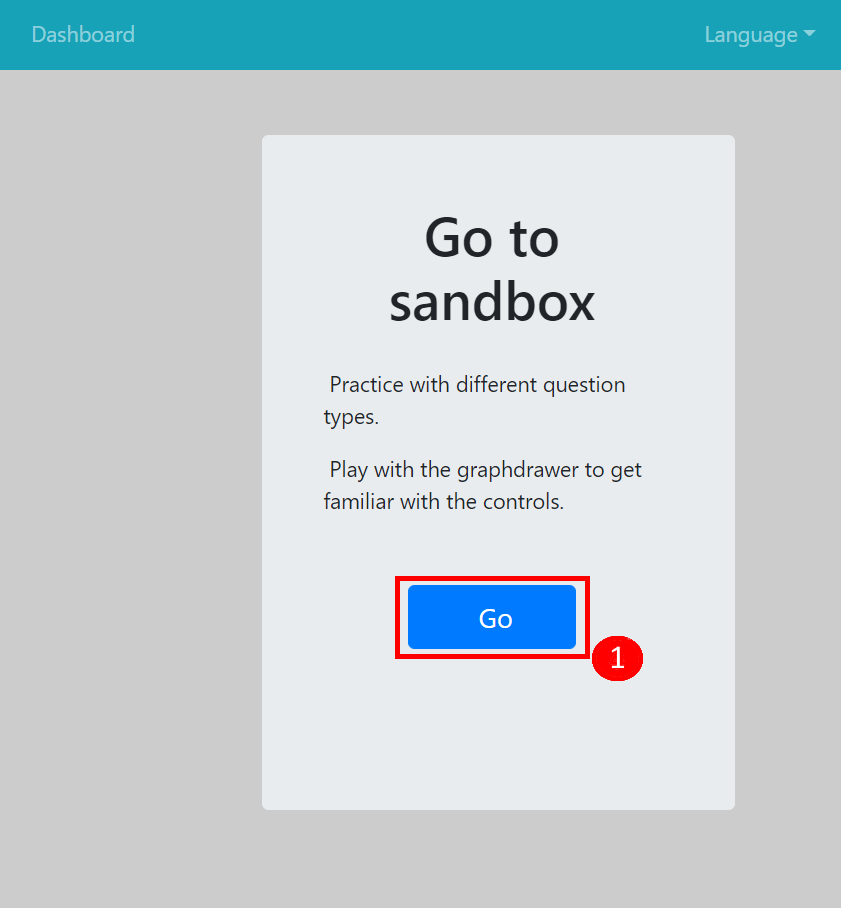
\includegraphics[width=\linewidth]{userManual/client/sandbox/goToSandbox}
		\caption{}
		\label{fig:goToSanbox}
	\end{subfigure}
	\begin{subfigure}{0.80\linewidth}
		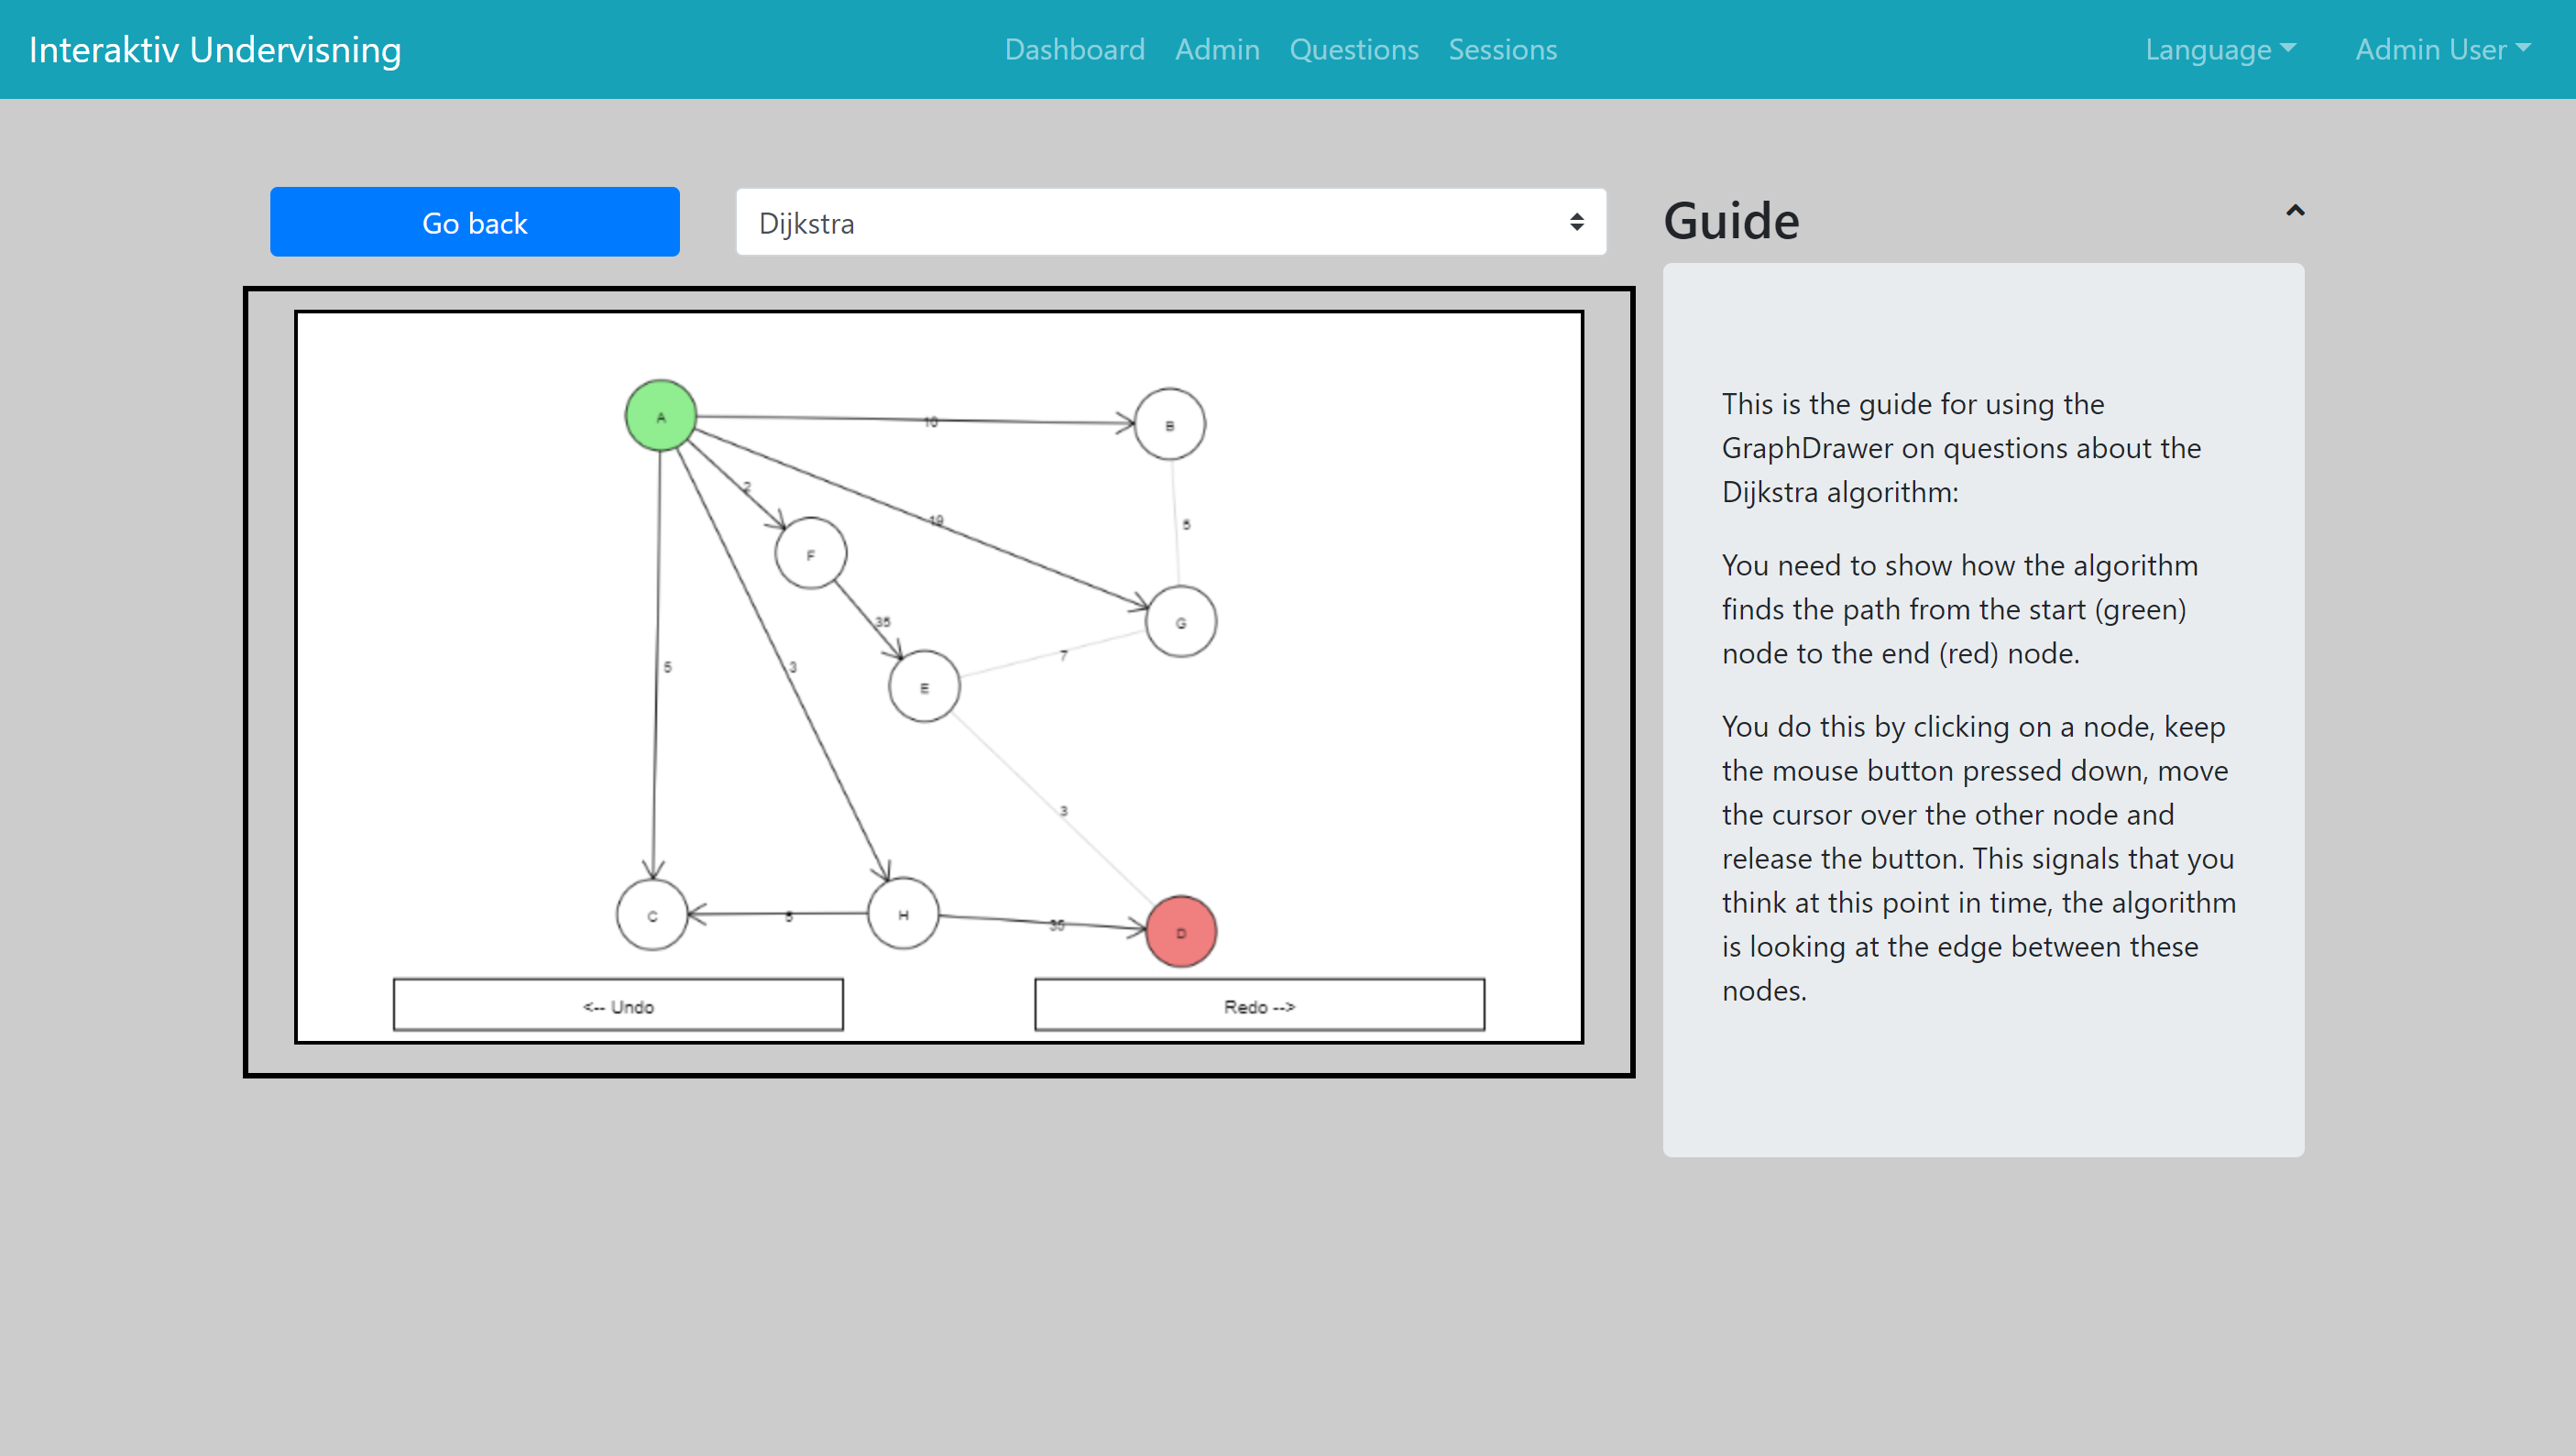
\includegraphics[width=\linewidth]{userManual/client/sandbox/sandbox}
		\caption{}		
		\label{fig:sandbox}
	\end{subfigure}
\end{figure}

\begin{userManualItemlist}
	\item[Step I.] Navigate to the dashboard page.
	\item[Step II.] Click the button(1) labeled "Go" within the "Go to sandbox" area. (Figure: \ref{fig:goToSanbox})
	\item[Step III.] Select the question type you want to practise. (2) (Figure: \ref{fig:sandbox})
	\item[Step IV.] Read the user guide for the chosen question type. (3) (Figure: \ref{fig:sandbox})
	\item[Step IV.(2)] Some question types has access to a settings together with the user guide. If this is the case then you have the option of changing the question types initial settings. (Figure: \ref{fig:sandbox})
	\item[Step V.] Practise solving exercises with the given tools. (4) (Figure: \ref{fig:sandbox})
	\item[Step VI.] When you are finished exit the sandbox by clicking the button (5) labeled "Go back". (Figure: \ref{fig:sandbox})
\end{userManualItemlist}